\documentclass[11pt,a4paper]{article}

\usepackage[
    a4paper,
    left=15mm,
    right=15mm,
    top=30mm,
    bottom=25mm,
    headheight=25mm
]{geometry}
\usepackage{graphicx}
\usepackage{polski}
\usepackage[utf8]{inputenc}
\usepackage{enumerate}
\usepackage{comment}
\usepackage{fancyhdr}
\usepackage{hyperref}
\usepackage{indentfirst}
\usepackage{multirow}
\usepackage{multicol}
\usepackage{float}
\usepackage{amsmath}
\usepackage{fancyhdr}
\usepackage{wrapfig}
\usepackage{layout}
\usepackage{textcomp}
\usepackage[center]{caption}
\usepackage{subcaption}
\usepackage{siunitx}

\sisetup{output-exponent-marker=\ensuremath{\mathrm{e}}}

\renewcommand{\baselinestretch}{1.18}
\renewcommand\thesubfigure{\roman{subfigure}}

\pagestyle{fancy}
\fancyhead[L]{
    
\includegraphics[scale=0.16]{../agh_logo_text_asym.jpg}
}
\fancyhead[R]{
    Lab 4 - Przecinanie odcinków 
    | Łukasz Dragon 25.11.2024
}

\begin{document}
\section{Wstęp}
Celem ćwiczenia było zaimplementowanie algorytmu
szukającego przecięć w zadanym zbiorze odcinków
metodą "zamiatania".

\subsection{Wstęp teoretyczny}
Implementując algorytm przyjęliśmy następujące założenia:
\begin{itemize}
    \item Wszystkie odcinki leżą na jednej płaszczyźnie.
    \item Żaden odcinek nie jest pionowy (równoległy do osi $OY$).
    \item Współrzędne $x$ odcinków są parami różne.
    \item Odcinki przecinają się w co najwyżej jednym punkcie.
    \item W jednym punkcie przecinają się co najwyżej dwa odcinki.
\end{itemize}

Algorytm korzystał z metody "zamiatania", 
przesuwając "miotłę" (prostą równoległą do osi $OY$)
w miejsce kolejnych zdarzeń trzymanych w strukturze $Q$
i aktualizując strukturę stanu $T$, przetrzymującą odcinki
obecnie przecinające się z miotłą.

\subsubsection{Struktura zdarzeń $Q$}
Zdarzeniami w algorytmie są początki, końce oraz miejsca
przecięć odcinków posortowane rosnąco względem współrzędnej $x$.
Struktura ta musi wspierać szybkie dodawanie nowych zdarzeń oraz
odczyt kolejnego zdarzenia.

W mojej implementacji algorytmu strukturą zdarzeń jest
drzewo czerwono-czarne, na którym operacje dodawania i odczytu
wykonywane są ze złożonością obliczeniową $O(logn)$, gdzie $n$ 
oznacza liczbę elementów w drzewie. Użyłem właśnie tej struktury
aby uniknąć dodawania dwukrotnie tego samego przecięcia jako zdarzenia;
algorytm przed dodaniem zdarzenia sprawdza, czy w strukturze zdarzeń
już się ono nie znajduje (zdarzenia jesteśmy w stanie rozróżnić
przechowując czy reprezentują początek, koniec lub przecięcie odcinków 
oraz indeksy odcinków do których się odnosi). 
Z tego powodu także program nigdy nie usuwa zdarzeń, 
jedynie przechodząc do kolejnego.

Inną stukturą, która mogła być wykorzystana jest przykładowo
kolejka priorytetowa, a w przypadku algorytmu sprawdzającego
tylko czy istnieje przecięcie, wystarzy użycie odpowiednio
posortowanej listy (algorytm ten nie dodaje nigdy zdarzeń).

\subsubsection{Struktura stanu $T$}
Stan programu reprezentowany jest przez zbiór odcinków
obecnie zamiatanych przez miotłę, posortowany względem
współrzędnej $y$ punktu przecięcia z miotłą.
Struktura ta musi wspierać szybkie dodawanie, usuwanie
oraz odczyt odcinków.

Podobnie jak dla $Q$, w mojej implementacji strukturą stanu
jest drzewo czerwono-czarne. Program przechowuje w niej 
indeksy zamiatanych odcinków porównując je funkcją, która
oblicza ich punkty przecięcia z miotłą. Użycie takiej funkcji
porównującej sprawia, że struktura nie musi na nowo sortować
wartości po dodaniu nowej. Kolejność dwóch odcinków w strukturze 
zmienia się jedynie w miejscu ich przecięcia, co pozwala nam
je wtedy zamienić miejscami, bez zmieniania wewnętrznej struktury
drzewa.

\subsubsection{Algorytm zamiatania}
Algorytm obsługuje kolejno zdarzenia ze struktury $Q$
w następujący sposób:
\begin{itemize}
    \item Jeżeli zdarzenie jest początkiem odcinka, 
    to dodajemy go do $T$. Następnie sprawdzamy
    czy przecina się on z odcinkami sąsiadującymi
    w strukturze stanu.
    \item Jeżeli zdarzenie jest końcem odcinka,
    to usuwamy go z $T$ i sprawdzamy czy jego byli
    sąsiedzi przecinają się ze sobą.
    \item Jeżeli zdarzenie jest przecięciem odcinków,
    to zamieniamy ich kolejność w strukturze stanu,
    a następnie sprawdzamy czy przecinają się z ich 
    nowymi sąsiadami.
\end{itemize}
We wszystkich przypadkach, jeżeli znajdziemy dwa 
przecinające się odcinki, to dodajemy nowe zdarzenie
do $Q$, sprawdzając czy wcześniej już go nie dodaliśmy
(aby uniknąc sprawdzania wielokrotnie tego samego przecięcia).
Przeciecie odcinków znajdujemy przyrównując postacie kierunkowe
prostych przechodzących przez początki i końce odcinków i sprawdzając
czy znaleziony punkt zawiera się w obu odcinkach.

Ostatecznie wynikiem programu jest lista trójek zawierających
współrzędne przecięcia oraz indeksy przecinających się odcinków.

~

\begin{tabular}{l|l|l}
    Złożoność obliczeniowa: & $O((p + n)logn)$ & \footnotesize gdzie $n$ oznacza liczbę odcinków,\\
    Złożoność pamięciowa: & $O(p + n)$ & \footnotesize a $p$ oznacza liczbę przecięć.\\
\end{tabular}  

\subsection{Specyfikacja narzędzi i sprzętu}
Wszystkie potrzebne obliczenia zostały wykonane przy użyciu interpretera języka Python wersji 3.12.
Ponadto, w celu wygenerowania zbiorów punktów użyłem biblioteki \verb|numpy|. 
Wykresy i wizualizacja wyników została przygotowana za pomocą narzędzia
przygotowanego przez koło naukowe Bit. Do implementacji interaktywnego
zadawania odcinków użyłem biblioteki \verb|matplotlib|. Kod znajduje się w załączonym pliku.
Przedstawione wyniki zostały wygenerowane na komputerze z systemem operacyjnym Debian 12 i 
procesorem AMD Ryzen 5 3600 3.6GHz.

\section{Realizacja obliczeń}
Realizację ćwiczenia zacząłem od implementacji struktury drzewa 
czerwono-czarnego oraz implementacji dwóch wersji 
omawianego algorytmu: \verb|is_intersection|, sprawdzającą czy 
istnieje jakiekolwiek przecięcie oraz \verb|find_intersections|,
szukającą wszystkich przecięć. 
Następnie dodałem do programu możliwość zadawania własnych 
odcinków za pomocą myszki lub generacji losowych zbiorów odcinków.
Ostatecznie przygotowałem cztery zbiory testowe, sprawdzające czy
algorytm działa poprawnie w danych przypadkach. Zbiory te przedstawione
są na Rysunku 1.

\begin{figure}[H]
    \centering
    \begin{subfigure}[b]{0.46\textwidth}
        \centering
        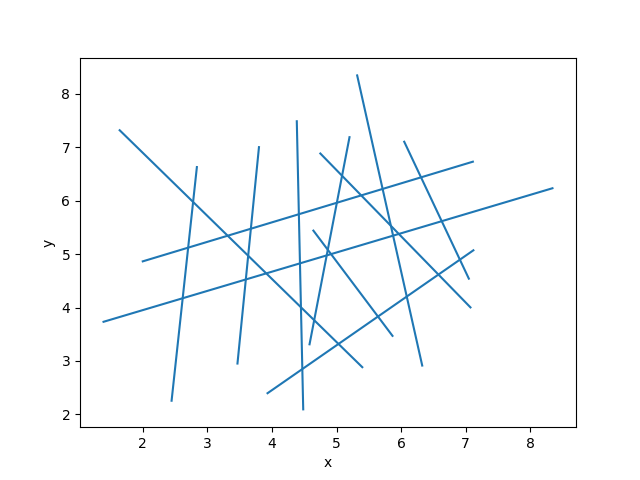
\includegraphics[scale=0.4]{res/sec_a.png}
        \caption{
            Zbiór A
        }
    \end{subfigure}
    \begin{subfigure}[b]{0.46\textwidth}
        \centering
        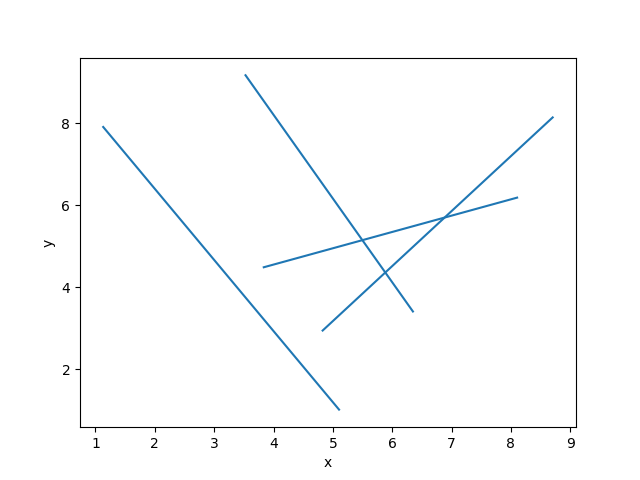
\includegraphics[scale=0.4]{res/sec_b.png}
        \caption{
            Zbiór B
        }
    \end{subfigure}
    \begin{subfigure}[b]{0.46\textwidth}
        \centering
        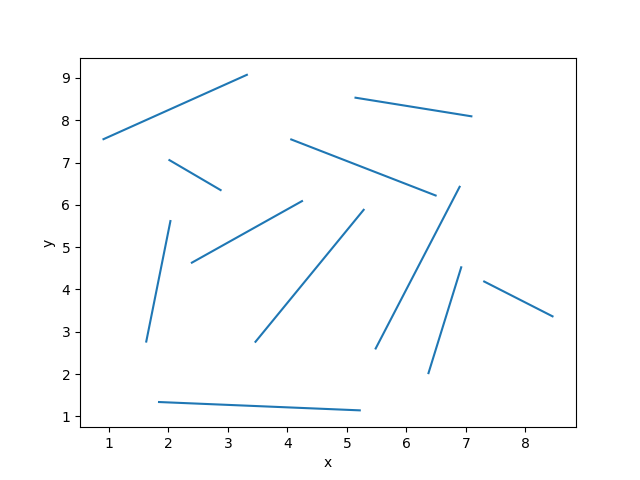
\includegraphics[scale=0.4]{res/sec_c.png}
        \caption{
            Zbiór C
        }
    \end{subfigure}
    \begin{subfigure}[b]{0.46\textwidth}
        \centering
        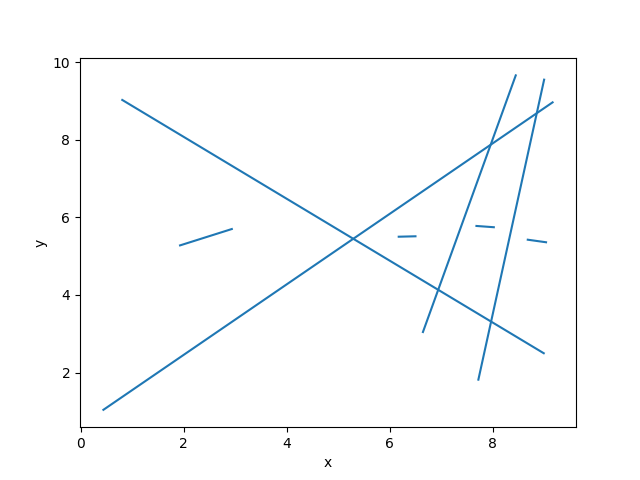
\includegraphics[scale=0.4]{res/sec_d.png}
        \caption{
            Zbiór D
        }
    \end{subfigure}
    \caption{Wybrane zbiory testowe}
\end{figure}

\section{Wyniki dla zbiorów testowych}
Sekcje od 3.1 do 3.4 zawierają ilustracje wyników działania
algorytmu dla zbiorów testowych wraz z krótkim komentarzem
na temat tego co testują. Algorytm \verb|is_intersection|
zwraca wartość \verb|True| jeżeli istnieje conajmniej jedno
przecięcie lub \verb|False| w przeciwnym przypadku.
Rysunki 2, 3, 4, 5 zawierają znalezione
przez algorytm \verb|find_indersections| 
przecięcia oznaczone kolorem czerwonym.
Ponadto, razem ze sprawozdaniem zawarte są animacje
pokazujące kolejne kroki działania algorytmu dla każdego 
zbioru. W animacjach przyjmuję następujące oznaczenia:
\begin{itemize}
    \item Kolor niebieski - odcinki, do których miotła jeszcze nie doszła.
    \item Kolor zielony - odcinki w strukturze stanu.
    \item Kolor żółty - odcinki, między którymi algorytm obecnie szuka przeciecia.
    \item Kolor szary - odcinki sprawdzone, poza strukturą stanu.
    \item Punkty czerwone - znalezione punkty przeciecia.
    \item Czerwona linia - obecna pozycja miotły.
\end{itemize}
Zawarty ze sprawozdaniem kod wypisuje także znalezione
przeciecia w formie tekstowej.

\subsection{Zbiór A}
Zbiór testuje czy algorytm znajdzie wszystkie przecięcia
w przypadku gdzie wszystkie odcinki przecinają się 
conajmniej z trzema innymi.

Wyniki:

\verb|is_intersectiom|: \verb|True|

\begin{figure}[H]
    \centering
    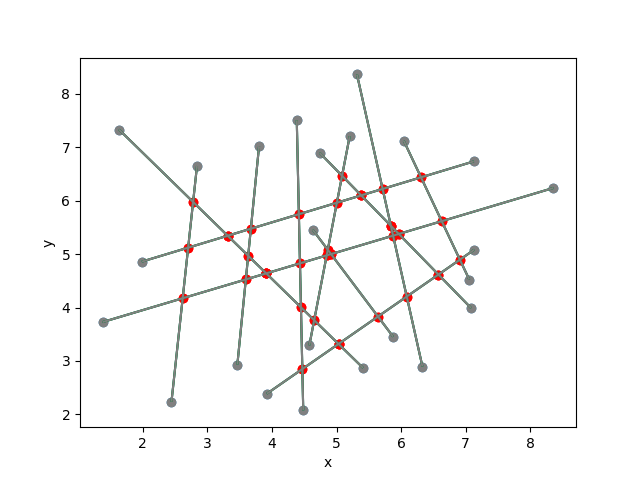
\includegraphics[scale=0.5]{res/int_a.png}
    \caption{Ilustracja wyniku \ttfamily find\_intersections \normalfont dla \\zbioru A}
\end{figure}

\subsection{Zbiór B}
Zbiór testuje czy algorytm poprawnie działa dla małej
liczby przecięć oraz czy algorytm poprawnie sortuje strukturę
stanu.

Wyniki:

\verb|is_intersectiom|: \verb|True|

\begin{figure}[H]
    \centering
    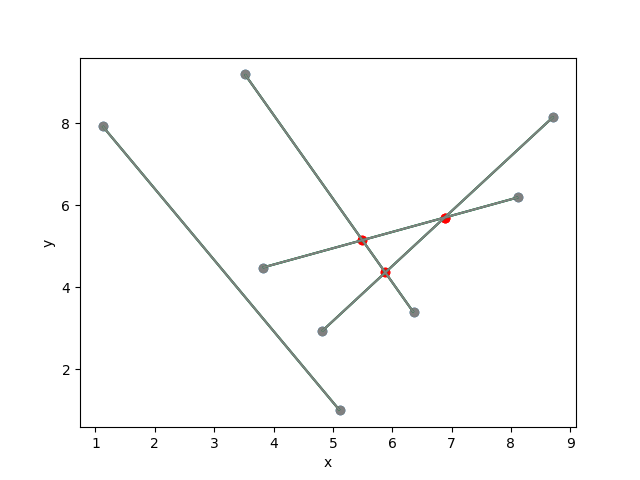
\includegraphics[scale=0.5]{res/int_b.png}
    \caption{Ilustracja wyniku \ttfamily find\_intersections \normalfont dla \\zbioru A}
\end{figure}

\subsection{Zbiór C}
Zbiór testuje czy algorytm poprawnie radzi sobie w przypadku,
w którym nie ma przecięć.

Wyniki:

\verb|is_intersectiom|: \verb|False|

\begin{figure}[H]
    \centering
    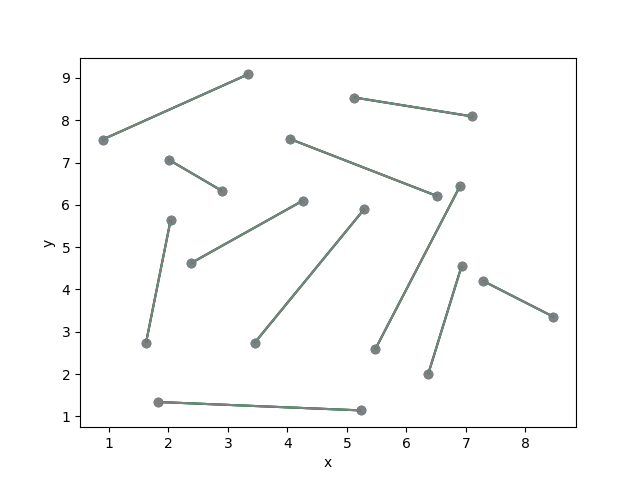
\includegraphics[scale=0.5]{res/int_c.png}
    \caption{Ilustracja wyniku \ttfamily find\_intersections \normalfont dla \\zbioru A}
\end{figure}

\subsection{Zbiór D}
Zbiór testuje czy algorytm poprawnie radzi sobie w przypadku,
w którym przecięcia wykrywane są więcej niż jeden raz.

Wyniki:

\verb|is_intersectiom|: \verb|True|

\begin{figure}[H]
    \centering 
    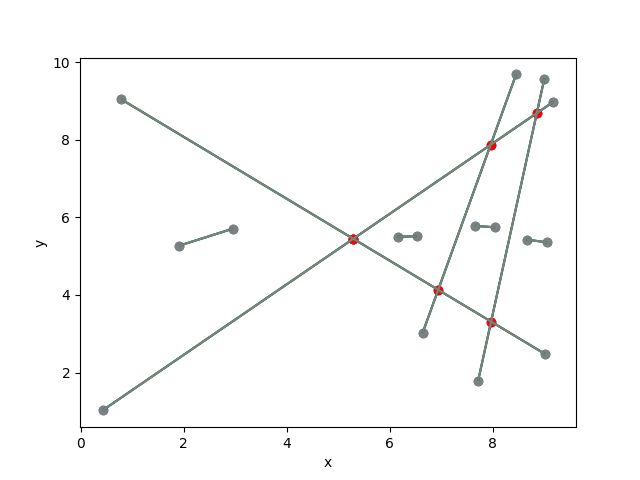
\includegraphics[scale=0.5]{res/int_d.png}
    \caption{Ilustracja wyniku \ttfamily find\_intersections \normalfont dla \\zbioru A}
\end{figure}

\section{Podsumowanie}
Zaimplementowane algorytmy przechodzą wybrane przeze mnie testy 
oraz te zawarte w narzędziu przygotowanym przez koło naukowe Bit.
Wygenerowane przez program wyniki oraz funkcjonalność losowania
lub zadawania własnych zbiorów jest zawarta w załączonym kodzie.
Wraz ze sprawozdaniem załączone są także wygenerowane przez program
animacje ilustrujące działanie algorytmu dla wybranych zbiorów testowych.

\end{document}
